%!TEX program = xelatex
\documentclass[dvipsnames,svgnames,a4paper,11pt]{article}

% -----------------------------------------------------
%	加边框的命令
%	参考：https://tex.stackexchange.com/questions/531559/how-to-add-the-page-border-for-first-two-pages-in-latex
\usepackage{tikz}
\usetikzlibrary{calc}
\usepackage{eso-pic}
\AddToShipoutPictureBG{%
\begin{tikzpicture}[overlay,remember picture]
\draw[line width=0.6pt] % 边框粗细
    ($ (current page.north west) + (0.6cm,-0.6cm) $)
    rectangle
    ($ (current page.south east) + (-0.6cm,0.6cm) $); % 边框位置
\end{tikzpicture}}


\usepackage{xcolor}
\definecolor{c1}{HTML}{2752C9} % 目录颜色
\definecolor{c2}{RGB}{190,20,83} % 引用颜色

\usepackage{ctex}
\usepackage[top=28mm,bottom=28mm,left=15mm,right=15mm]{geometry} % 调整边距
\usepackage{hyperref}
\hypersetup{
	colorlinks,
	linktoc = section, % 给目录加的超链接位置，选项有 section, page, all
	linkcolor = c1, % linkcolor 目录颜色
	citecolor = c1  % citecolor 引用颜色
}
\usepackage{amsmath,enumerate,multirow,float}
\usepackage{tabularx}
\usepackage{tabu}
\usepackage{subfig}
\usepackage{fancyhdr}
\usepackage{graphicx}
\usepackage{wrapfig}
\usepackage{physics}
\usepackage{appendix}
\usepackage{amsfonts,amssymb}
% \usepackage{annotate-equations} % 公式标注（未安装，已禁用）
\usepackage{pgfplots} % pgf 绘图


% ---------------------------------------------------------------------
%	定义了两类colorbox
\usepackage{tcolorbox}
\tcbuselibrary{skins,breakable}
\newtcolorbox{tbox}[2][]{
    colframe=black!70!,
    breakable,
    enhanced, % 跨页后不会显示下边框
    boxrule =0.5pt,
    title = {#2},
    fonttitle = \large\bfseries,
    drop fuzzy shadow,
    #1
}
\newtcolorbox[auto counter,number within=section]{question}[1][]{
  top=2pt,bottom=2pt,arc=1mm,
  boxrule=0.5pt,
  breakable,
  enhanced, % 跨页后不会显示下边框
  coltitle=c1!80!gray,
  colframe=c1,
  colback=c1!3!white,
  drop fuzzy shadow,
  title={思考题~\thetcbcounter：\quad},
  fonttitle=\bfseries,
  attach title to upper,
  #1
}

% ---------------------------------------------------------------------
%	利用 cleveref 改变引用格式，\cref 是引用命令
\usepackage{cleveref}
\crefformat{figure}{#2{\textcolor{c2}{图 #1}}#3} % 图片的引用格式
\crefformat{equation}{#2{(\textcolor{c2}{#1})}#3} % 公式的引用格式
\crefformat{table}{#2{\textcolor{c2}{表 #1}}#3} % 表格的引用格式

% ---------------------------------------------------------------------
%	页眉页脚设置
\fancypagestyle{plain}{\pagestyle{fancy}}
\pagestyle{fancy}
\lhead{\kaishu 中山大学物理与天文学院物理实验\uppercase\expandafter{\romannumeral3}} % 左边页眉，学院 + 课程
\rhead{\kaishu Template 实验报告模板} % 右边页眉，实验报告标题
\cfoot{\thepage} % 页脚，中间添加页码
\setlength{\headheight}{13.6pt}

% ---------------------------------------------------------------------
%	对目录、章节标题的设置
\renewcommand{\contentsname}{\centerline{\huge 目录}}
% titlesec/titletoc 与 ctex 冲突，已禁用
% \usepackage{titlesec}
% \usepackage{titletoc}
% \titleformat{\section}{\centering\LARGE}{}{1em}{}
% \newcommand{\nsection}[3]{%
%     \section{#1 #2 \hspace{11pt} \textbf{#3}}%
% }

% ---------------------------------------------------------------------
%   listing代码环境设置
\usepackage{listings}
\lstloadlanguages{python}
\lstdefinestyle{pythonstyle}{
backgroundcolor=\color{gray!5},
language=python,
frameround=tftt,
frame=shadowbox,
keepspaces=true,
breaklines,
columns=spaceflexible,
basicstyle=\ttfamily\small, % 基本文本设置，字体为 teletype，大小为 small
keywordstyle=[1]\color{c1}\bfseries,
keywordstyle=[2]\color{Red!70!black},
stringstyle=\color{Purple},
showstringspaces=false,
commentstyle=\ttfamily\scriptsize\color{green!40!black}, % 注释文本设置，字体为 teletype，大小为 scriptsize
tabsize=2,
morekeywords={as},
morekeywords=[2]{np, plt, sp},
numbers=left, % 代码行数，位置在左
numberstyle=\it\tiny\color{gray}, % 代码行数的数字字体设置
stepnumber=1,
rulesepcolor=\color{gray!30!white}
}


% ---------------------------------------------------------------------
%	将表格封装起来
\newcommand{\scoresTable}[8]{
    \begin{table}
        \renewcommand\arraystretch{1.7}
        \begin{tabularx}{\textwidth}{
                |X|X|X|X
                |X|X|X|X|}
            \hline
            \multicolumn{2}{|c|}{预习报告} & \multicolumn{2}{|c|}{实验记录} & \multicolumn{2}{|c|}{分析讨论} & \multicolumn{2}{|c|}{总成绩} \\
            \hline
            \centering#1&\centering#2 &\centering#3 &\centering#4 &\centering#5 &\centering#6 &\centering#7 &{\centering#8} \\
            \hline
        \end{tabularx}
    \end{table}
}
\newcommand{\infoTable}[6]{
    \begin{table}
        \renewcommand\arraystretch{1.7}
        \begin{tabularx}{\textwidth}{|X|X|X|X|}
        \hline
        专业：& #1 &年级：& #2\\
        \hline
        姓名：& #3   & 学号：&#4\\
        \hline
        实验时间：&#5 & 教师签名：&#6 \\
        \hline
        \end{tabularx}
    \end{table}
}

% ---------------------------------------------------------------------
%	其他设置
\def\degree{${}^{\circ}$} % 角度
\graphicspath{{./}{./images/}} % 插入图片的相对路径
\allowdisplaybreaks[4]  %允许公式跨页

\usetikzlibrary{patterns,decorations.markings,arrows.meta,bending} % TikZ 包的拓展

\pgfplotsset{compat=1.18}
\graphicspath{{./}{images/}}

\usepackage{booktabs}
\usepackage{longtable}
\usepackage{makecell}
\usepackage{array}
\usepackage{pdflscape}
\usepackage{enumitem}
\usepackage{caption}
\usetikzlibrary{positioning,shapes.geometric,calc,arrows.meta,backgrounds,fit}
\definecolor{hexBlue}{HTML}{4F7DFF}
\definecolor{hexBlueFill}{HTML}{DDE8FF}
\definecolor{hexGreen}{HTML}{39C849}
\definecolor{hexGreenFill}{HTML}{DCF8D9}
\definecolor{hexGray}{HTML}{B8BEC6}
\definecolor{hexGrayFill}{HTML}{F0F1F3}
\definecolor{hexYellow}{HTML}{FFE600}
\definecolor{hexYellowFill}{HTML}{FFFCC8}
\definecolor{hexOrange}{HTML}{FF8B2B}
\definecolor{hexOrangeFill}{HTML}{FCE7CA}
\definecolor{hexRed}{HTML}{FF5B5B}
\definecolor{hexRedFill}{HTML}{F8DDDD}
\definecolor{refcolor}{HTML}{4F7DFF}
\definecolor{textcolor}{HTML}{39C849}
\definecolor{synthcolor}{HTML}{FF8B2B}
\definecolor{voccolor}{HTML}{FF5B5B}

\hypersetup{
    pdftitle={实验一：Fashion-MNIST 分类与反向传播},
    pdfauthor={赵浩宇}
}
\lhead{\kaishu 计算机视觉实验报告}
\rhead{\kaishu 实验一：Fashion-MNIST}
\setlength{\parskip}{0.35em}
\setlength{\parindent}{2em}
\renewcommand{\arraystretch}{1.2}
\captionsetup{font=small,labelfont=bf}

\begin{document}
\ClearShipoutPictureBG
\begin{titlepage}
\thispagestyle{empty}
\begin{center}
    \vspace*{0.25cm}
    
\includegraphics[width=0.40\textwidth]{images/school_flat.png}\par
    \vspace{0.55cm}
    {\fontsize{30pt}{36pt}\selectfont\bfseries 计算机视觉\par}
    \vspace{0.65cm}
    {\fontsize{28pt}{34pt}\selectfont\bfseries 实验报告\par}
    \vspace{1.6cm}
    {\fontsize{22pt}{34pt}\selectfont\bfseries 实验一：Fashion-MNIST\par}
    {\fontsize{20pt}{30pt}\selectfont\bfseries 分类与反向传播\par}
\end{center}

\vspace{0.25cm}
\begin{center}
{\small \textbf{GitHub 代码地址：}\url{https://github.com/TakamiyaMioo/DeepLearning_Homework/tree/main/Fashion-MNIST%20Experiments}}
\end{center}
\vspace{0.2cm}
\begin{center}
\renewcommand\arraystretch{1.75}
{\fontsize{17pt}{23pt}\selectfont
\begin{tabular}{p{0.22\textwidth}p{0.48\textwidth}}
学院： & \underline{\makebox[0.36\textwidth][c]{电子信息与通信学院}} \\
专业班级： & \underline{\makebox[0.36\textwidth][c]{电信2303班}} \\
姓名： & \underline{\makebox[0.36\textwidth][c]{赵浩宇}} \\
学号： & \underline{\makebox[0.36\textwidth][c]{U202314553}} \\
指导教师： & \underline{\makebox[0.48\textwidth][c]{王兴刚、廖振宇、闫增强}} \\
\end{tabular}
}
\end{center}
\end{titlepage}

\begingroup
\renewcommand{\contentsname}{\centerline{\LARGE 目录}}
\small
\setlength{\parskip}{0pt}
\tableofcontents
\endgroup
\clearpage

\section{实验目的}

本实验围绕 Fashion-MNIST 十分类任务，完成以下工作：
\begin{enumerate}[leftmargin=2em]
  \item 将官方训练集按固定随机种子划分为训练集和验证集，保留官方测试集用于最终评价。
  \item 实现线性 Softmax 分类器，记录训练与验证曲线，并分析测试准确率、混淆矩阵、逐类召回率和分类错误。
  \item 仅使用 NumPy 在固定小批量上实现单隐层 MLP 的前向计算和反向传播，用中心差分检查梯度。
  \item 在统一训练条件下比较线性分类器、无激活的两层线性模型和带 ReLU 的 MLP。
  \item 针对训练中观察到的验证损失后期回升现象提出假设，通过只改变最大训练轮数的对照实验检验该假设。
\end{enumerate}

\section{数据集与实验设置}

Fashion-MNIST 包含 70,000 张 $28\times28$ 的灰度图像，分为 10 个服饰类别；官方训练集有 60,000 张，官方测试集有 10,000 张\cite{fashionmnist}。本实验用固定划分种子 42 对官方训练集随机排列，将前 50,000 个索引作为训练集、其余 10,000 个索引作为验证集。划分索引保存并供所有模型共同使用，因此不同模型的训练数据和验证数据一致。官方测试集仅在模型按验证集准确率选定检查点后用于最终评价。

图像通过 \texttt{ToTensor} 转换为 $[0,1]$ 浮点张量，不使用随机增强。数据划分由固定 split seed 42 产生并缓存，训练、验证和测试数据的用途严格分离。三模型比较分别使用训练种子 42、123 和 2026；每次训练均训练 30 个 epoch，batch size 为 128，优化器为 Adam，学习率为 $10^{-3}$，weight decay 为 0。训练数据加载器以固定 split seed 初始化 shuffle generator，因此不同模型使用同一训练样本顺序；模型初始化则按各自训练种子执行。每个 epoch 含 391 个 mini-batch（最后一批 80 个样本），每次完整训练共 11,730 次参数更新。测试准确率和 Macro-F1 报告三种子均值及样本标准差。训练曲线、线性分类器混淆矩阵、逐类召回率、错误样本图以及诊断图使用 seed 42 的对应运行。

正式训练运行在服务器 NVIDIA GeForce RTX 3080 Ti 上，Python 3.8、PyTorch 1.10.0+cu113 和 torchvision 0.11.1+cu113。服务器驱动提供 CUDA GPU 运行时，无需在实验中安装 CUDA Toolkit。

\section{原理分析}

\subsection{线性 Softmax 分类器}

将一个批次的图像展平为 $X\in\mathbb{R}^{B\times784}$。线性层计算类别分数
\[
  Z=XW+b,\qquad W\in\mathbb{R}^{784\times10},\quad b\in\mathbb{R}^{10}.
\]
对每行分数作 Softmax 得到
\[
  p_{ic}=\frac{\exp(z_{ic})}{\sum_{j=1}^{10}\exp(z_{ij})},
\]
训练目标为批次平均交叉熵
\[
  \mathcal{L}=-\frac{1}{B}\sum_{i=1}^{B}\log p_{i,y_i}.
\]
实现中先对分数减去每行最大值，再计算指数和对数，以减少数值溢出。该模型共有 $784\times10+10=7,850$ 个可训练参数。

\subsection{NumPy 单隐层 MLP 与反向传播}

NumPy 检查使用固定合成小批量 $X\in\mathbb{R}^{4\times4}$、5 个隐藏单元和 3 个输出类别。隐藏层使用 $\tanh$：
\[
 A=XW_1+b_1,\qquad H=\tanh(A),\qquad Z=HW_2+b_2.
\]
输出层使用 Softmax 交叉熵。令 $P$ 为预测概率矩阵、$Y$ 为 one-hot 标签矩阵，则
\[
 \frac{\partial\mathcal{L}}{\partial Z}=\frac{P-Y}{B},\quad
 \frac{\partial\mathcal{L}}{\partial W_2}=H^\mathsf{T}\frac{\partial\mathcal{L}}{\partial Z},\quad
 \frac{\partial\mathcal{L}}{\partial b_2}=\sum_i\frac{\partial\mathcal{L}}{\partial Z_i}.
\]
继续向前传播梯度，
\[
 \frac{\partial\mathcal{L}}{\partial H}=\frac{\partial\mathcal{L}}{\partial Z}W_2^\mathsf{T},\qquad
 \frac{\partial\mathcal{L}}{\partial A}
 =\frac{\partial\mathcal{L}}{\partial H}\odot(1-H\odot H),
\]
\[
 \frac{\partial\mathcal{L}}{\partial W_1}=X^\mathsf{T}\frac{\partial\mathcal{L}}{\partial A},\qquad
 \frac{\partial\mathcal{L}}{\partial b_1}=\sum_i\frac{\partial\mathcal{L}}{\partial A_i}.
\]
对每个参数元素使用中心差分
\[
 g_{\mathrm{num}}(\theta)=
 \frac{\mathcal{L}(\theta+\epsilon)-\mathcal{L}(\theta-\epsilon)}{2\epsilon},
 \qquad \epsilon=10^{-5},
\]
并计算解析梯度和数值梯度的相对 $L_2$ 误差。检查在 float64 下完成，容许阈值为 $10^{-6}$。该实验只验证实现，不使用 NumPy 训练整个 Fashion-MNIST 数据集。

相对误差的具体定义为
\[
  e_{\mathrm{rel}}=\frac{\|g_{\mathrm{ana}}-g_{\mathrm{num}}\|_2}
  {\|g_{\mathrm{ana}}\|_2+\|g_{\mathrm{num}}\|_2+10^{-12}}.
\]
本次检查以随机种子 42 生成输入、标签和参数；对 $W_1,b_1,W_2,b_2$ 的所有元素逐个扰动，因此结果不依赖抽样挑选参数坐标。

\subsection{受控比较模型}

PyTorch 中的三个模型结构如下。两层线性模型与 ReLU MLP 使用相同的隐藏宽度 128。

\begin{table}[H]
\centering
\caption{模型结构及可训练参数量}
\begin{tabular}{lll}
\toprule
模型 & 计算结构 & 参数量 \\
\midrule
Linear & $784\rightarrow10$ & 7,850 \\
Two-layer linear & $784\rightarrow128\rightarrow10$，无中间激活 & 101,770 \\
ReLU MLP & $784\rightarrow128\rightarrow\mathrm{ReLU}\rightarrow10$ & 101,770 \\
\bottomrule
\end{tabular}
\end{table}

对照实验固定数据划分、预处理、优化器、学习率、weight decay、batch size、训练轮数、验证集选模规则和三个训练种子，仅改变网络结构。无激活两层线性模型与 ReLU MLP 的隐藏宽度和参数量相同，两者之间的结构差异仅为是否使用 ReLU；这组对照用于考察非线性激活的作用。无激活模型与单层 Linear 的函数类别相同，但参数化和优化路径不同，因此二者差异不能解释为新增表达能力的效果。

无激活的两层线性模型可合成为一个仿射映射：
\[
 (xW_1+b_1)W_2+b_2=x(W_1W_2)+(b_1W_2+b_2).
\]
因此增加线性层本身不会增加非线性表达能力；它采用因子化参数化，优化过程与单层参数化不同。ReLU MLP 则通过非线性激活获得更灵活的决策边界。

\section{软件实现与结果}

\subsection{训练流程与模型选择}

所有 PyTorch 模型统一输出 logits，并采用交叉熵损失。每个 epoch 结束后计算验证损失和验证准确率，并按最高验证准确率保存检查点；准确率相同时保留更早的 epoch。测试集仅用于所选检查点的最终指标。训练过程开启 PyTorch 确定性算法设置；三种子实验共享同一数据划分、训练样本顺序和优化配置。随机种子、软件版本和运行命令列于项目 README，原始逐次运行指标及配置随项目结果文件保存。线性基线 seed 42 的完整运行耗时为 125.39 秒，其余模型和种子结果见\cref{tab:compare}。

\subsection{线性基线训练曲线与测试表现}

seed 42 的线性分类器在第 26 个 epoch 达到最高验证准确率 0.8608；对应测试准确率为 0.8476，测试 Macro-F1 为 0.8468。训练损失持续下降，验证损失在中后期下降趋缓并有小幅波动，验证准确率在约 0.85 至 0.86 间变化。\cref{fig:linearcurve} 展示训练与验证曲线。

\begin{figure}[H]
\centering
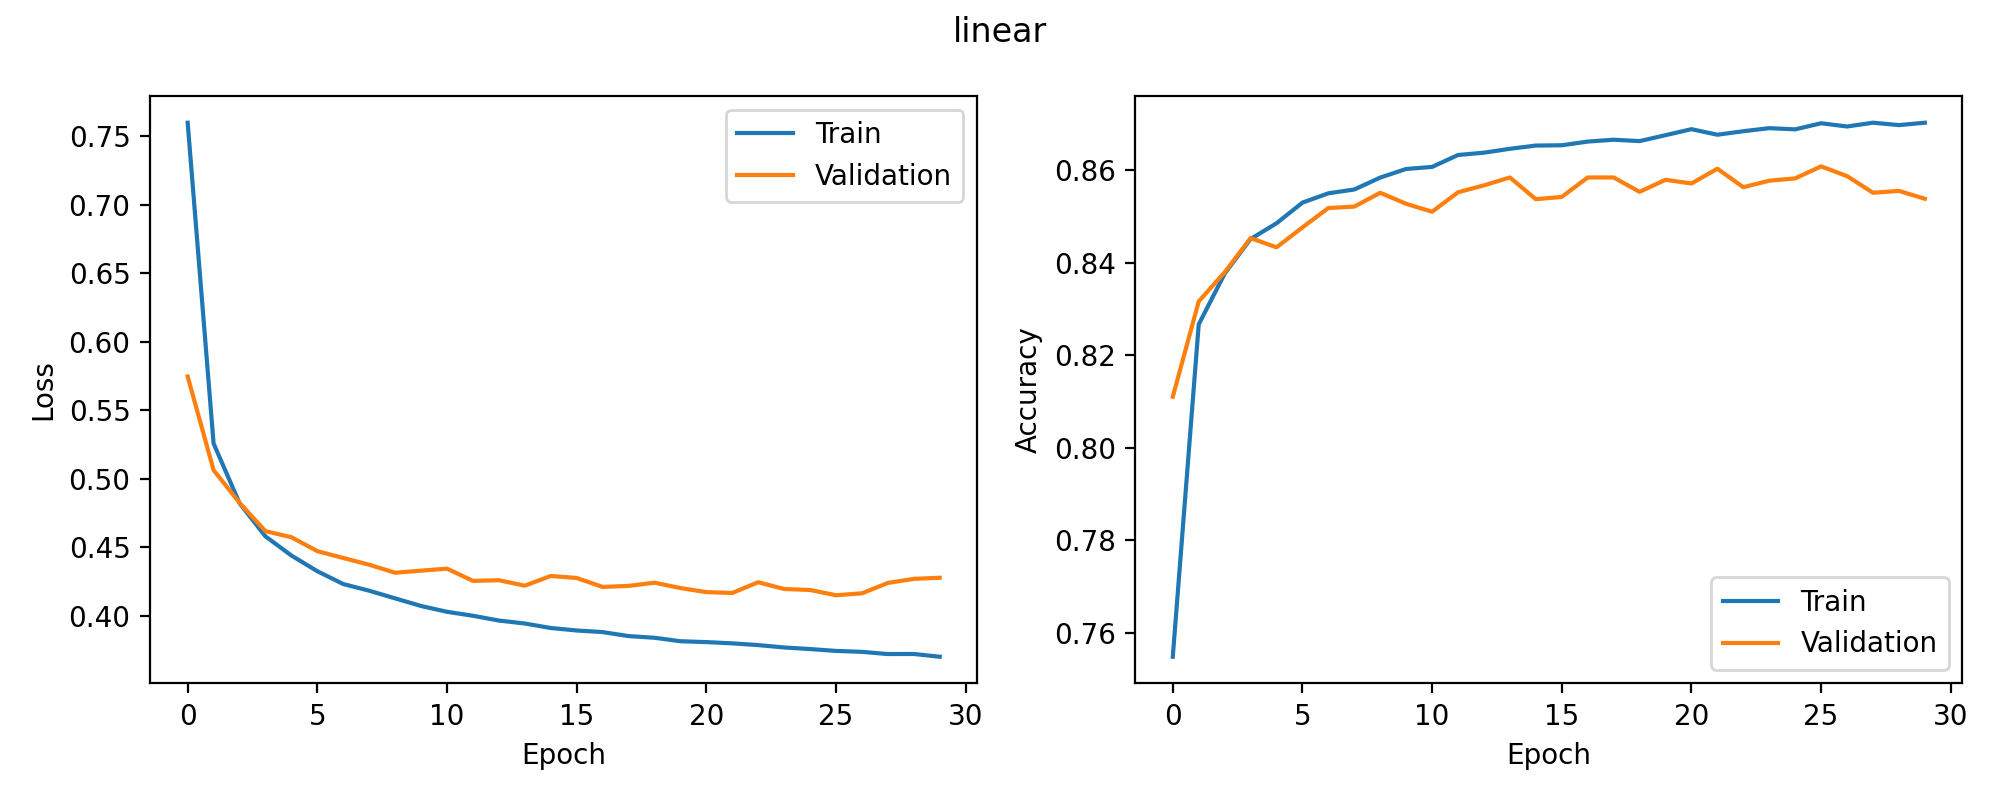
\includegraphics[width=0.98\textwidth]{images/exp1/linear_training.png}
\caption{线性 Softmax 分类器训练与验证曲线（seed 42）}
\label{fig:linearcurve}
\end{figure}

\subsection{线性基线混淆矩阵与逐类召回率}

\cref{fig:linearcm} 给出测试集混淆矩阵，矩阵每行对应真实类别、每列对应预测类别。测试集中每类有 1,000 张图像。混淆矩阵的对角线表示正确分类数；错误主要集中在外观相近的上衣类别之间。

\begin{figure}[H]
\centering
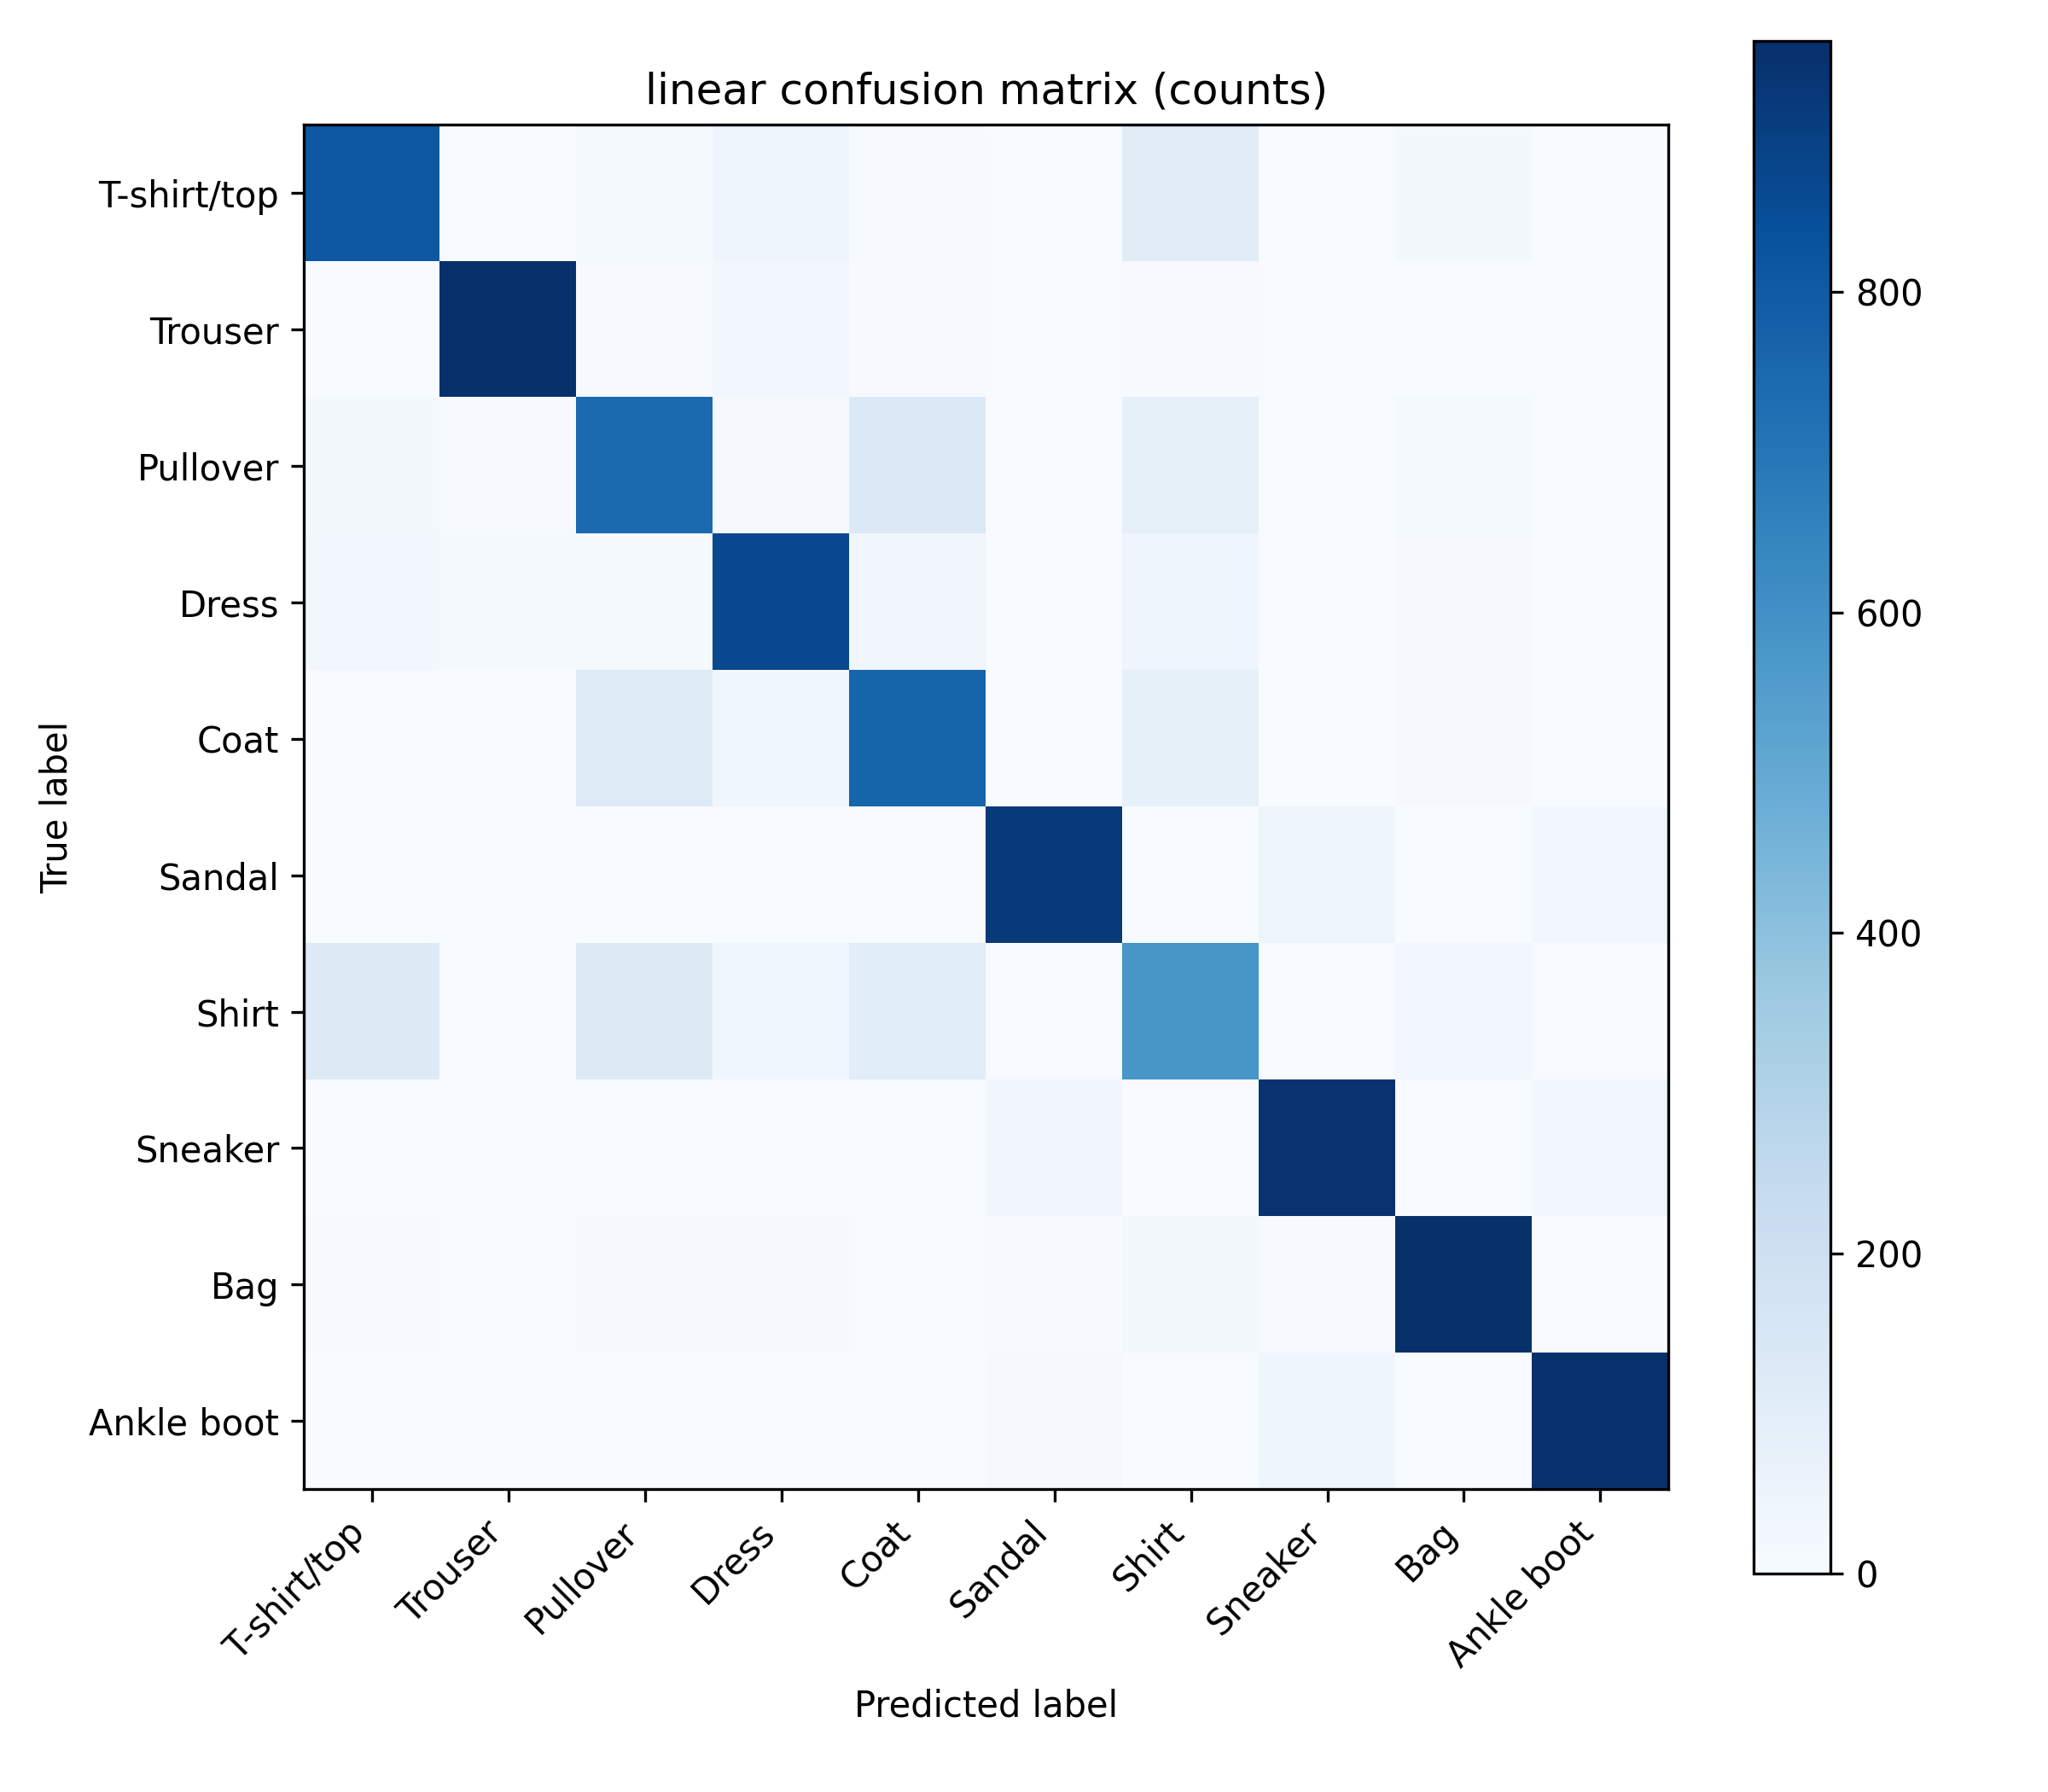
\includegraphics[width=0.82\textwidth]{images/exp1/linear_confusion.png}
\caption{线性 Softmax 分类器测试集混淆矩阵（seed 42）}
\label{fig:linearcm}
\end{figure}

\begin{table}[H]
\centering
\caption{线性基线逐类召回率（seed 42）}
\label{tab:recall}
\begin{tabular}{lrlr}
\toprule
类别 & 召回率 & 类别 & 召回率 \\
\midrule
T-shirt/top（上衣） & 0.810 & Trouser（裤子） & 0.957 \\
Pullover（套衫） & 0.743 & Dress（连衣裙） & 0.864 \\
Coat（外套） & 0.759 & Sandal（凉鞋） & 0.922 \\
Shirt（衬衫） & 0.578 & Sneaker（运动鞋） & 0.945 \\
Bag（包） & 0.952 & Ankle boot（短靴） & 0.946 \\
\bottomrule
\end{tabular}
\end{table}

\cref{tab:recall} 显示 Shirt 召回率最低，为 0.578；Trouser、Bag、Sneaker 和 Ankle boot 均高于 0.94。矩阵中较多的错误包括 Pullover 被判为 Coat（131 张）、Coat 被判为 Pullover（118 张），以及 Shirt 被判为 T-shirt/top 或 Pullover（各 127 张）。这与展平像素上的线性决策边界表达能力有限相符，但混淆矩阵本身只能显示错误分布，不能单独证明其成因。

\subsection{典型错误可视化}

\cref{fig:linearerrors} 展示按测试集固定顺序出现的前 16 个错误样本，并标出真实类别、预测类别和预测置信度。样例中包括 Sneaker 与 Sandal 混淆、Coat 与 Pullover 混淆，以及 Ankle boot 被判为 Sneaker。图像低分辨率且服饰轮廓相似时，类别边界并不总能从整体轮廓中明确分开；置信度较高也不代表分类正确。

\begin{figure}[H]
\centering
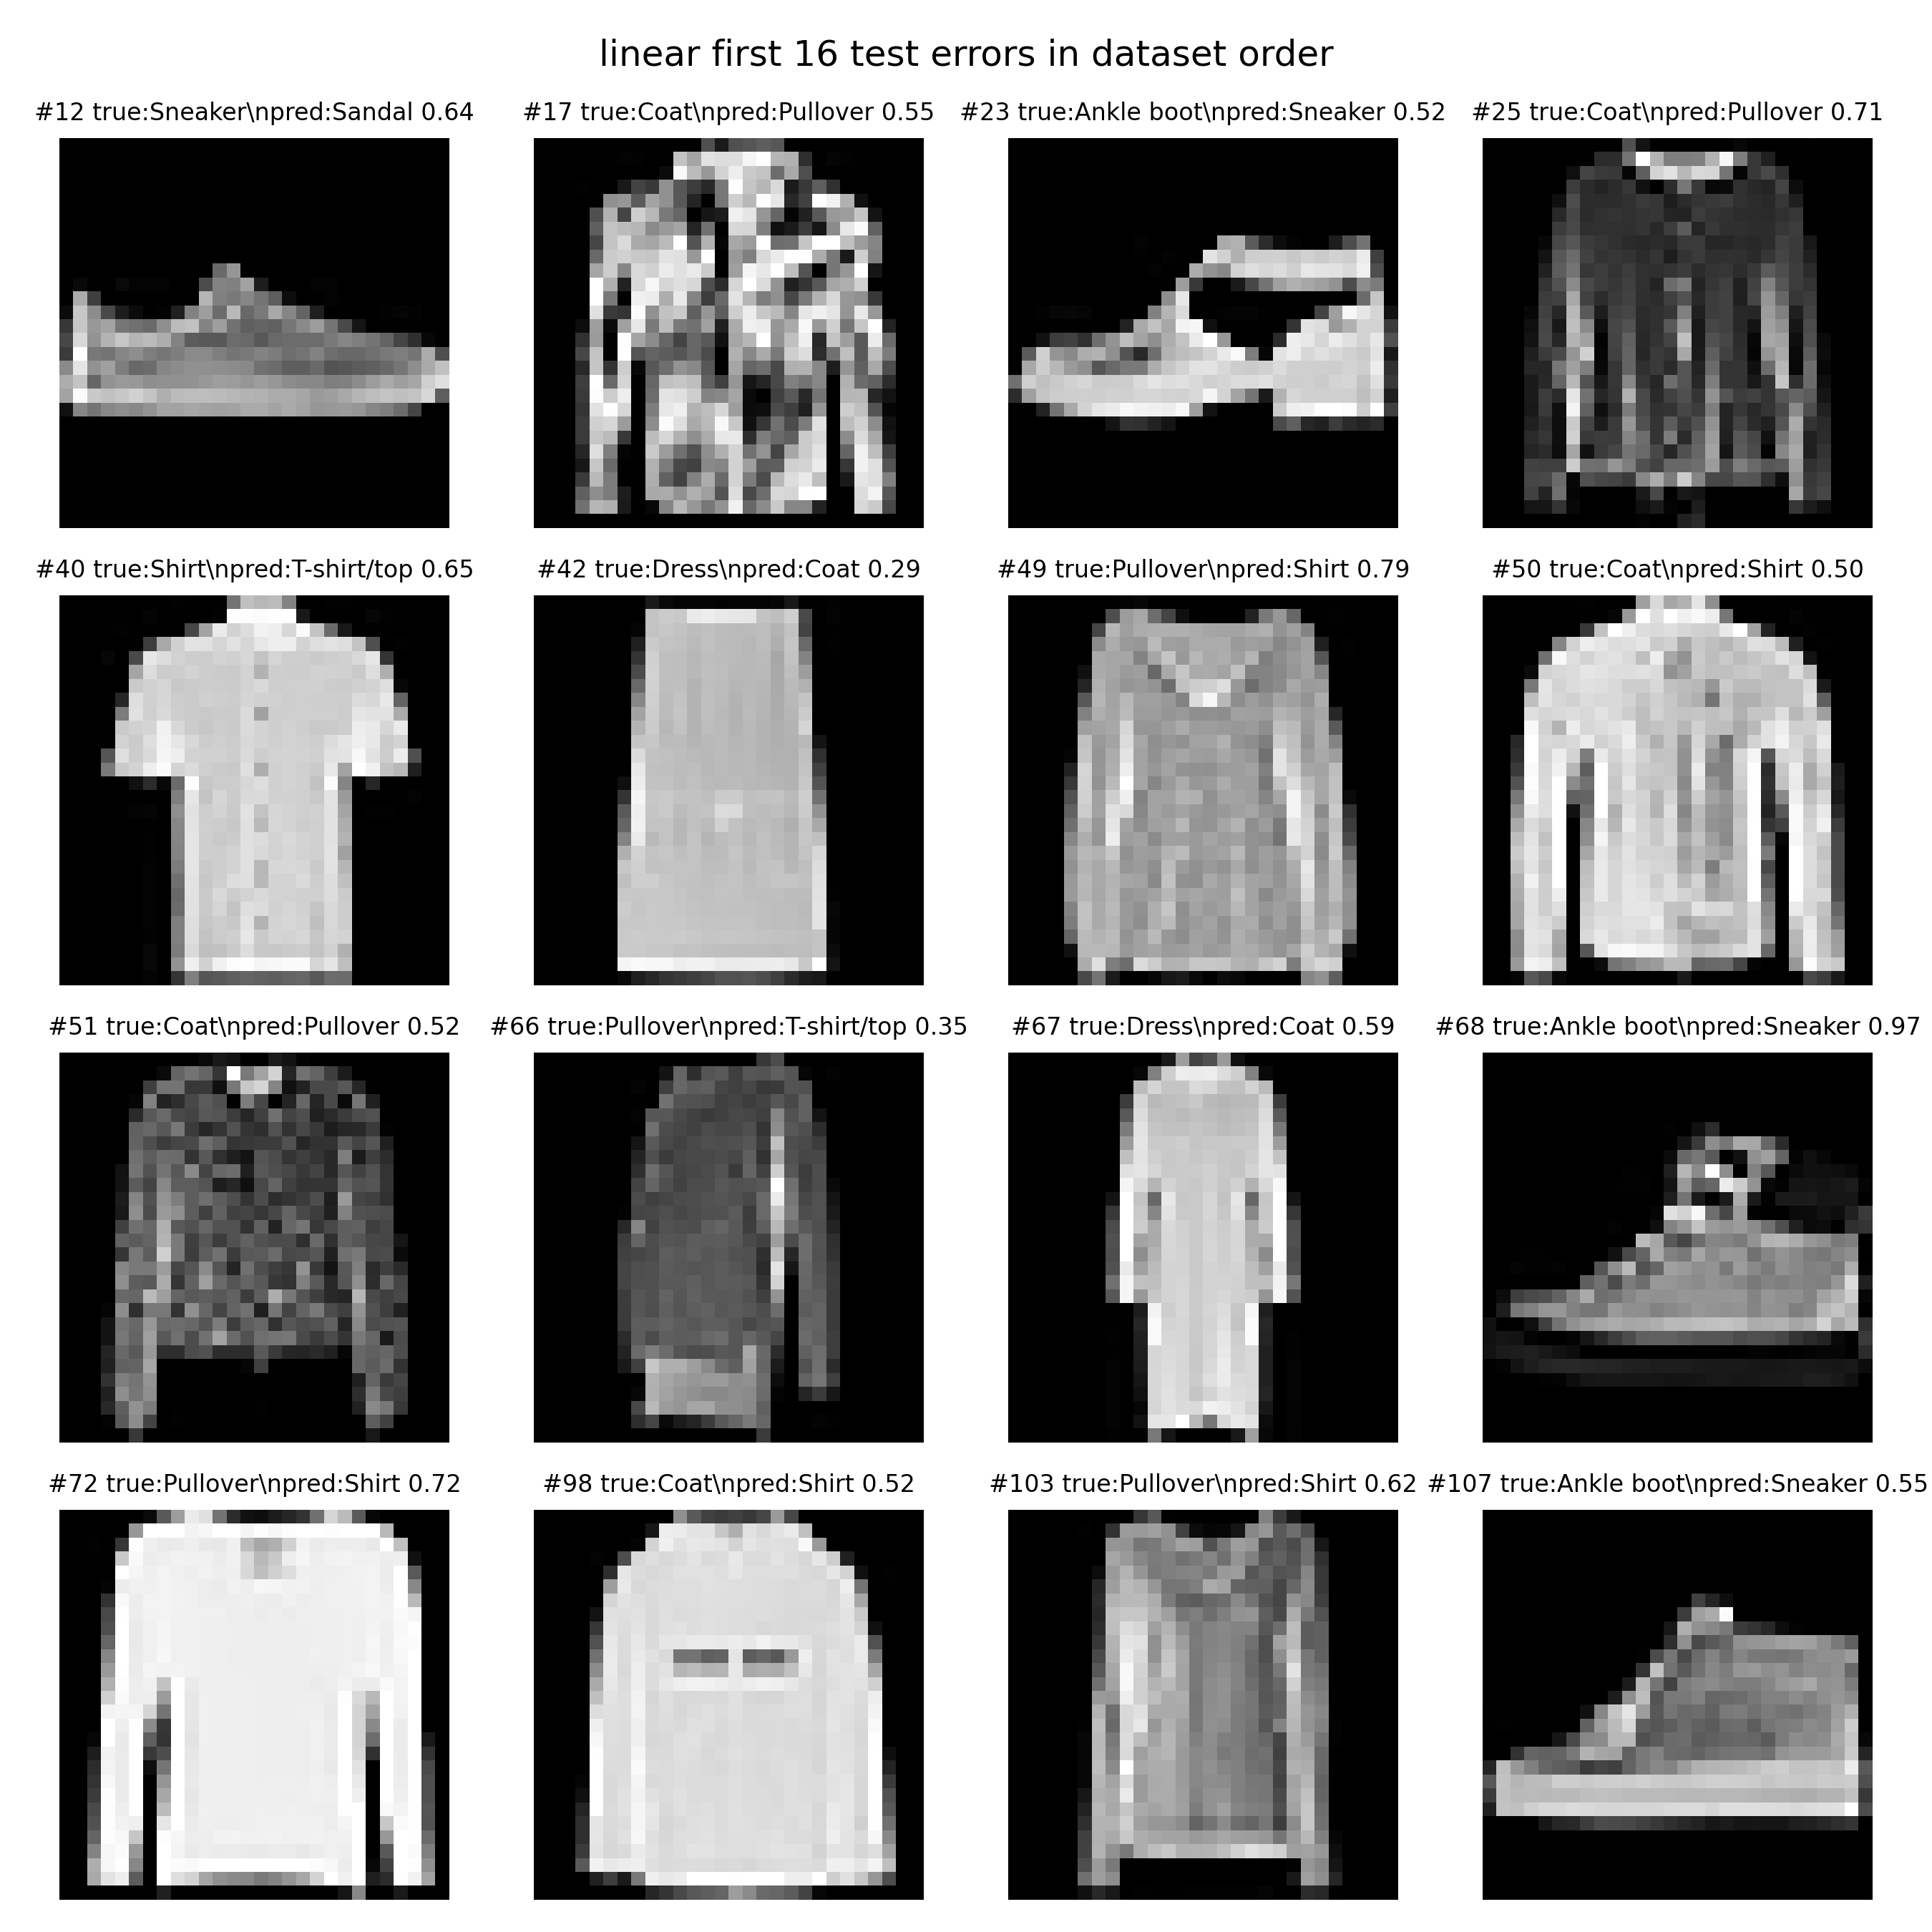
\includegraphics[width=0.94\textwidth]{images/exp1/linear_misclassified.png}
\caption{线性基线在测试集上的前 16 个错误样本，按测试集索引顺序选取}
\label{fig:linearerrors}
\end{figure}

\subsection{NumPy 梯度检查}

梯度检查逐元素比较反向传播解析梯度与中心差分数值梯度。共检查 43 个参数元素，四组参数的相对误差均远小于 $10^{-6}$ 阈值，检查通过。误差汇总见\cref{tab:grad} 和\cref{fig:grad}。

\begin{table}[H]
\centering
\caption{NumPy MLP 中心差分梯度检查结果}
\label{tab:grad}
\begin{tabular}{lrrrc}
\toprule
参数 & 检查元素数 & 最大绝对误差 & 相对误差 & 结果 \\
\midrule
$W_1$ & 20 & $1.82\times10^{-11}$ & $4.62\times10^{-10}$ & 通过 \\
$b_1$ & 5 & $6.51\times10^{-12}$ & $2.35\times10^{-10}$ & 通过 \\
$W_2$ & 15 & $1.34\times10^{-11}$ & $2.08\times10^{-10}$ & 通过 \\
$b_2$ & 3 & $7.58\times10^{-12}$ & $2.05\times10^{-11}$ & 通过 \\
\bottomrule
\end{tabular}
\end{table}

\begin{figure}[H]
\centering
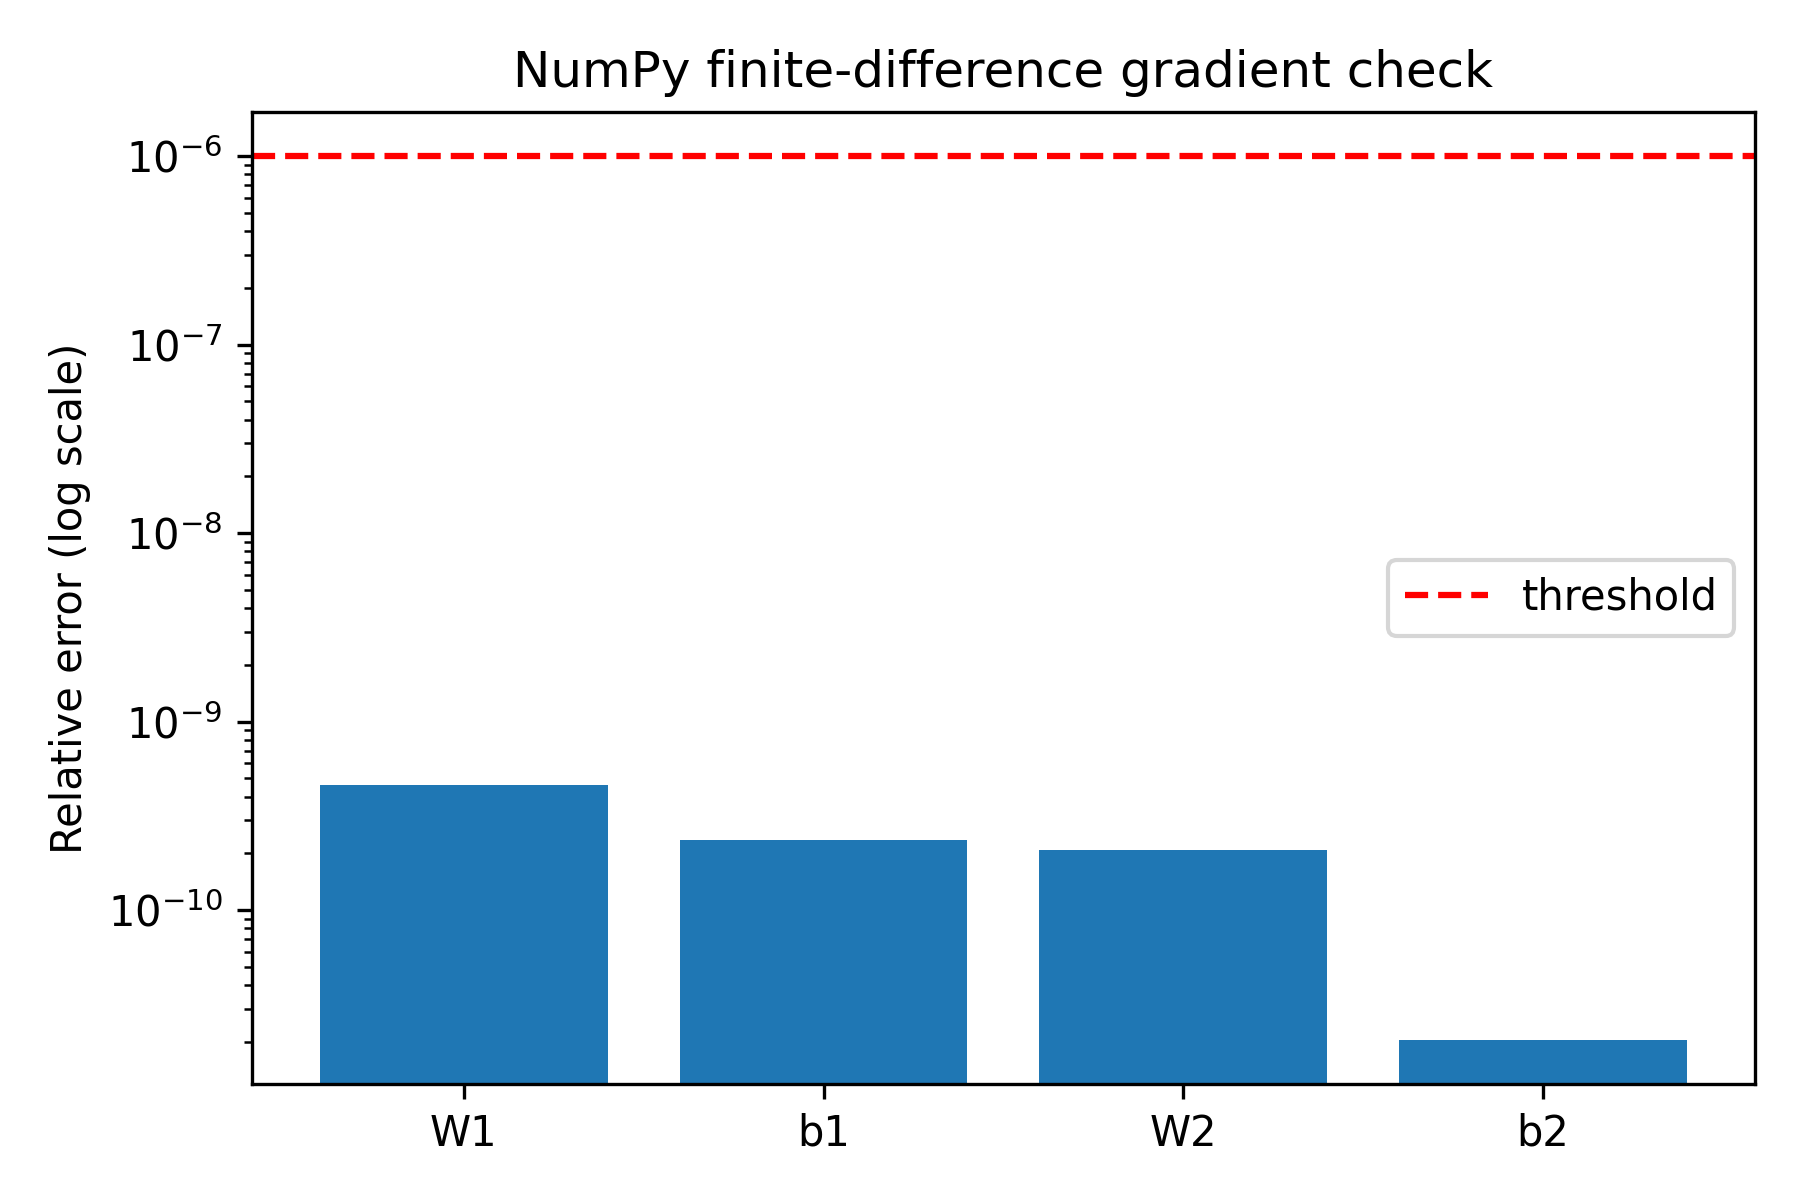
\includegraphics[width=0.82\textwidth]{images/exp1/gradient_check.png}
\caption{解析梯度与中心差分梯度的相对误差；红色虚线为 $10^{-6}$ 阈值}
\label{fig:grad}
\end{figure}

\subsection{三模型受控比较}

\cref{tab:compare} 汇总三个模型在 3 个训练种子上的均值和样本标准差。ReLU MLP 的平均测试准确率为 0.8840，较 Linear 的 0.8478 高 3.63 个百分点，较参数量相同的 Two-layer linear 高 3.96 个百分点；后一个差值是更直接的激活函数对照。逐种子看，ReLU MLP 相对 Linear 的测试准确率均高 3.55--3.77 个百分点，相对 Two-layer linear 均高 3.83--4.14 个百分点，方向在三个种子上保持一致。Macro-F1 的均值分别从 Linear 的 0.8469、Two-layer linear 的 0.8444 提升到 0.8846。seed 42/123/2026 下，ReLU MLP 对 Two-layer linear 的准确率差依次为 4.14/3.90/3.83 个百分点，说明观察到的差异并非由某一个种子单独造成。样本标准差描述这三个种子间的波动，不是置信区间；种子数只有 3，不能据此做强统计显著性结论。

Linear 有 7,850 个参数，而两个隐藏层模型各有 101,770 个，约为 Linear 的 13 倍。因此 ReLU MLP 相对 Linear 的优势同时包含更大的参数预算与非线性；相同参数量的 ReLU MLP 与 Two-layer linear 对比更能支持“加入非线性有帮助”的结论。无激活模型略低于单层 Linear 并不矛盾：相同仿射函数类下，分解参数化仍会改变 Adam 的优化轨迹。三模型完整运行耗时均值约为 122--125 秒，但计时区间包含训练、每轮验证、检查点保存和最终测试；在当前 GPU、软件和数据加载配置下没有观察到明显的运行时差别，不能将这些数字视为模型纯计算量的基准。

按 seed 42 的测试集逐类召回率，ReLU MLP 将 Shirt 从 0.578 提高到 0.765、Pullover 从 0.743 提高到 0.831；但 T-shirt/top 从 0.810 降至 0.789，Coat 则基本不变（0.759 对 0.761）。错误方向也有变化：Pullover 被判为 Coat 从 131 张降为 57 张，而 Coat 被判为 Pullover 仍有 116 张；T-shirt/top 被判为 Shirt 则由 107 张增至 153 张。这说明非线性模型总体减少错误、改善部分难分类类别，但不会均匀改善所有类别，类别间混淆也会重新分配。

\begin{table}[H]
\centering
\caption{三模型性能比较（3 个训练种子，均值 $\pm$ 样本标准差；完整运行时间包含训练、验证、检查点保存及最终测试）}
\label{tab:compare}
\small
\begin{tabular}{lrrrrr}
\toprule
模型 & 参数量 & 最佳验证准确率 & 测试准确率 & Macro-F1 & \makecell{完整运行\\时间（秒）} \\
\midrule
Linear & 7,850 & $0.8609\pm0.0003$ & $0.8478\pm0.0006$ & $0.8469\pm0.0006$ & $123.2\pm2.1$ \\
Two-layer linear & 101,770 & $0.8561\pm0.0008$ & $0.8445\pm0.0005$ & $0.8444\pm0.0005$ & $124.8\pm3.7$ \\
ReLU MLP & 101,770 & $0.8916\pm0.0009$ & $0.8840\pm0.0012$ & $0.8846\pm0.0018$ & $122.5\pm0.9$ \\
\bottomrule
\end{tabular}
\end{table}

\begin{figure}[H]
\centering
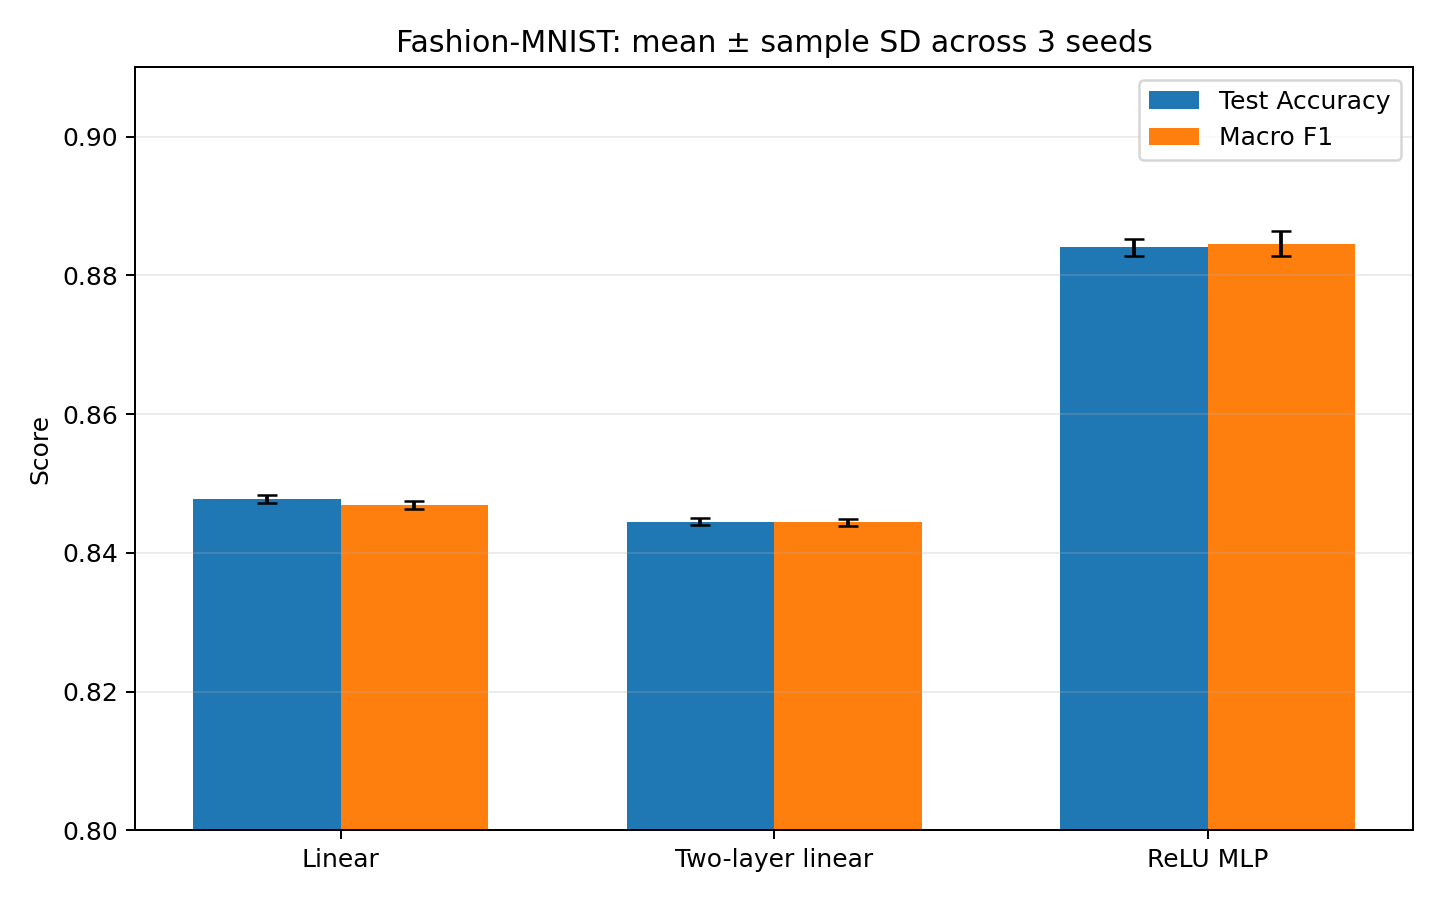
\includegraphics[width=0.82\textwidth]{images/exp1/model_comparison.png}
\caption{三模型测试准确率与 Macro-F1，误差线表示三个种子的样本标准差}
\label{fig:comparison}
\end{figure}

\begin{figure}[H]
\centering
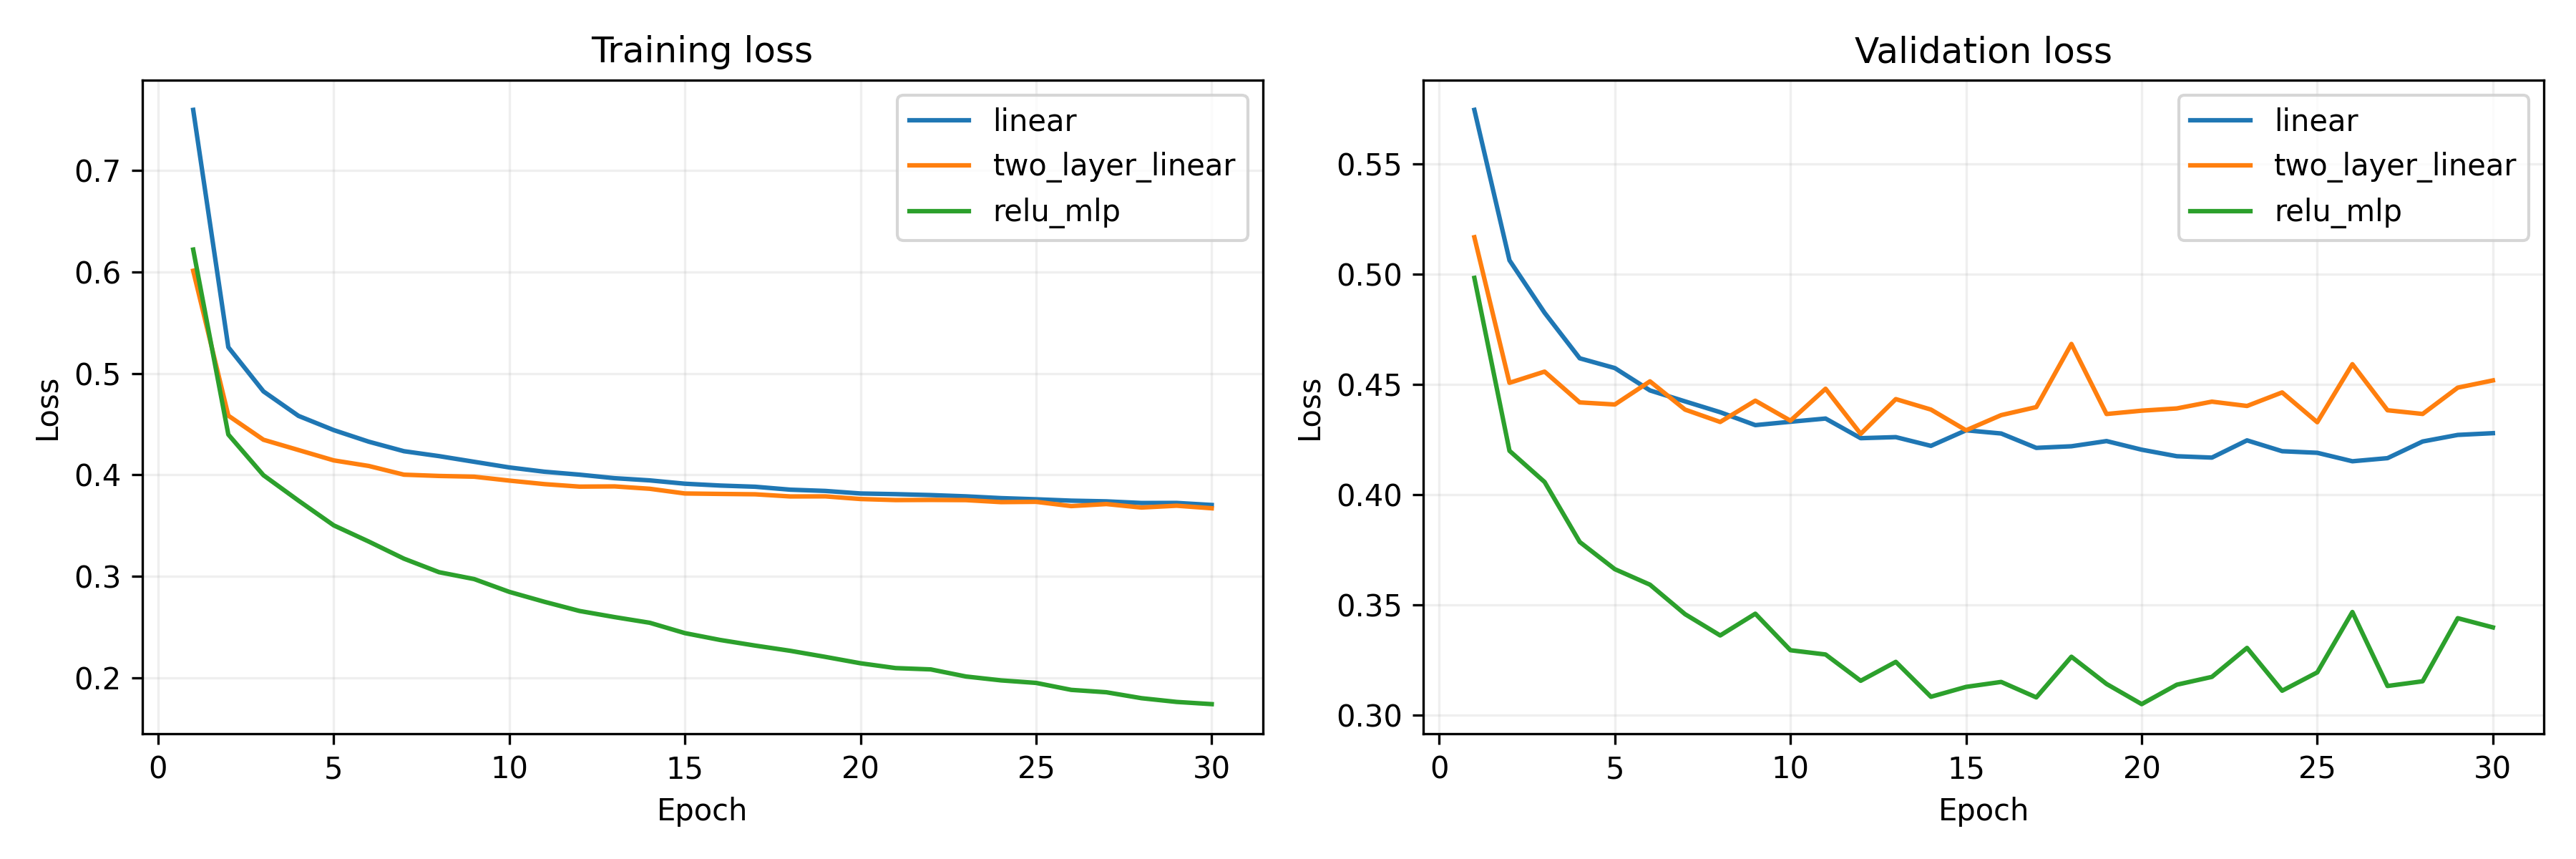
\includegraphics[width=0.96\textwidth]{images/exp1/three_models_loss.png}
\caption{三模型训练损失与验证损失曲线（seed 42）}
\label{fig:modelloss}
\end{figure}

\begin{figure}[H]
\centering
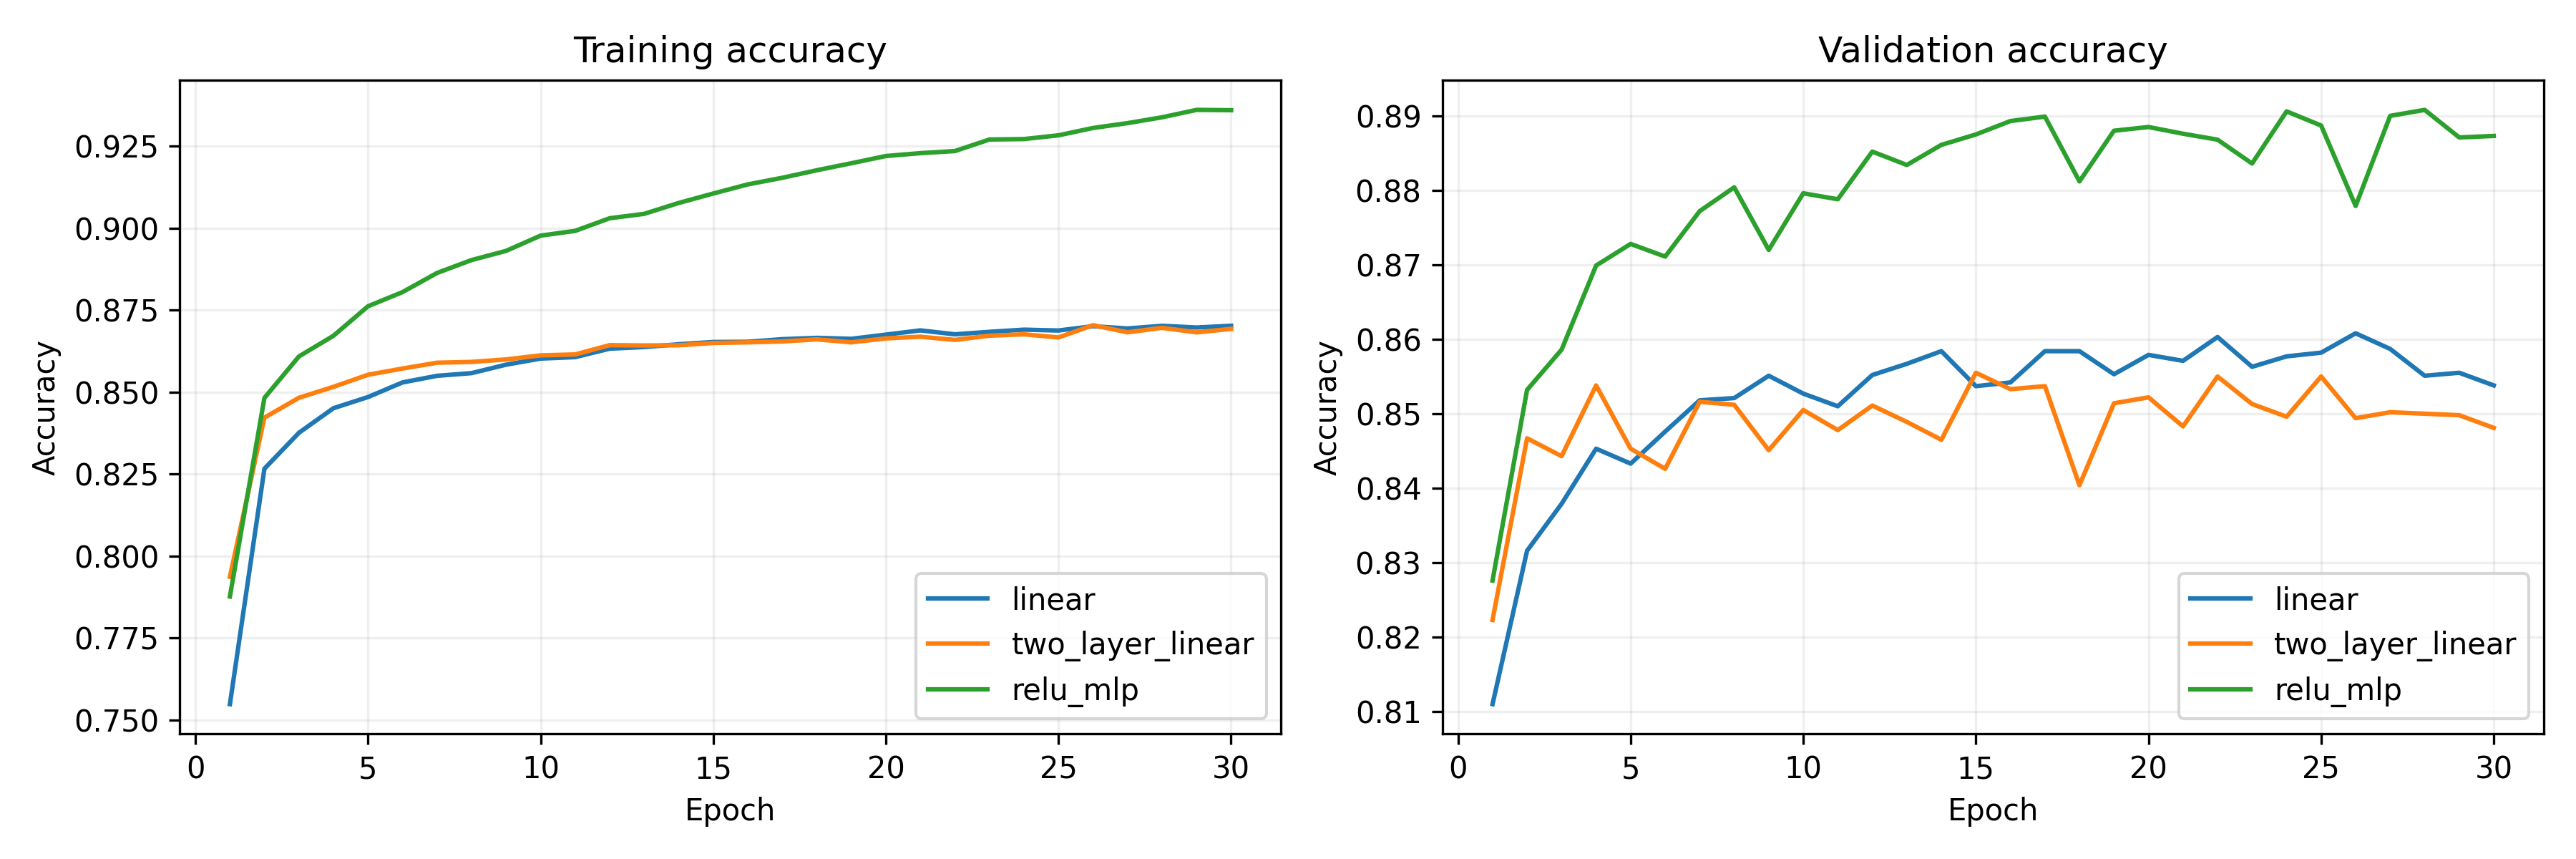
\includegraphics[width=0.96\textwidth]{images/exp1/three_models_accuracy.png}
\caption{三模型训练准确率与验证准确率曲线（seed 42）}
\label{fig:modelacc}
\end{figure}

\section{训练诊断：验证损失后期回升}

\subsection{观察与假设}

seed 42 的 ReLU MLP 训练损失从第 20 轮的 0.2143 继续降至第 30 轮的 0.1740，但验证损失从第 20 轮最低值 0.3049 回升至第 30 轮的 0.3397。训练准确率仍持续上升。一个可能解释是模型后期对训练样本拟合增强，出现过拟合；另一个需要保留的解释是验证集上少数困难或误分类样本的预测置信度变高，使交叉熵上升，而整体准确率变化较小。因此这里先称为“训练/验证损失分离”这一现象及过拟合假设，而不是仅凭损失曲线认定过拟合。

\subsection{单因素对照与结果}

验证假设时只改变最大训练轮数：控制组训练 30 轮，处理组训练 20 轮；随机种子、初始化、数据划分、优化器、学习率 $10^{-3}$、batch size 128 和 weight decay 均保持一致。处理组只用验证集选择检查点，不计算测试指标。两组第 1--20 轮的训练和验证记录完全一致，处理组实质上是相同训练轨迹在第 20 轮截断，因此该比较检验的是“是否继续训练”这一选择，而非两种独立训练策略的差异。结果如下：
\begin{itemize}[leftmargin=2em]
  \item 控制组（30 轮）最佳验证准确率为 0.8908（第 28 轮），全程最低验证损失为 0.3049（第 20 轮）。
  \item 处理组（20 轮）最佳验证准确率为 0.8899（第 17 轮），最低验证损失为 0.3049（第 20 轮）。
\end{itemize}
\cref{fig:diagnosticloss} 展示验证损失，\cref{fig:diagnosticacc} 展示训练准确率（两组至第 20 轮完全重合）。控制组验证准确率第 20 轮为 0.8885、第 28 轮达到最高值 0.8908、第 30 轮为 0.8873；处理组最高值为 0.8899（第 17 轮）。20 轮截断时验证损失达到与 30 轮组相同的最低值，但会错过第 28 轮略高的验证准确率。该结果显示延长训练降低了训练损失并提高了部分后期检查点的验证准确率，却未能阻止验证交叉熵回升；这更支持对模型置信度和损失变化继续检查，而非声称 20 轮明确优于 30 轮。单种子、单个截断点不能确认过拟合的具体机制，也不能证明缩短训练改善了测试泛化；该实验改变的是固定训练轮数上限，并非带 patience 的自动早停。

\begin{figure}[H]
\centering
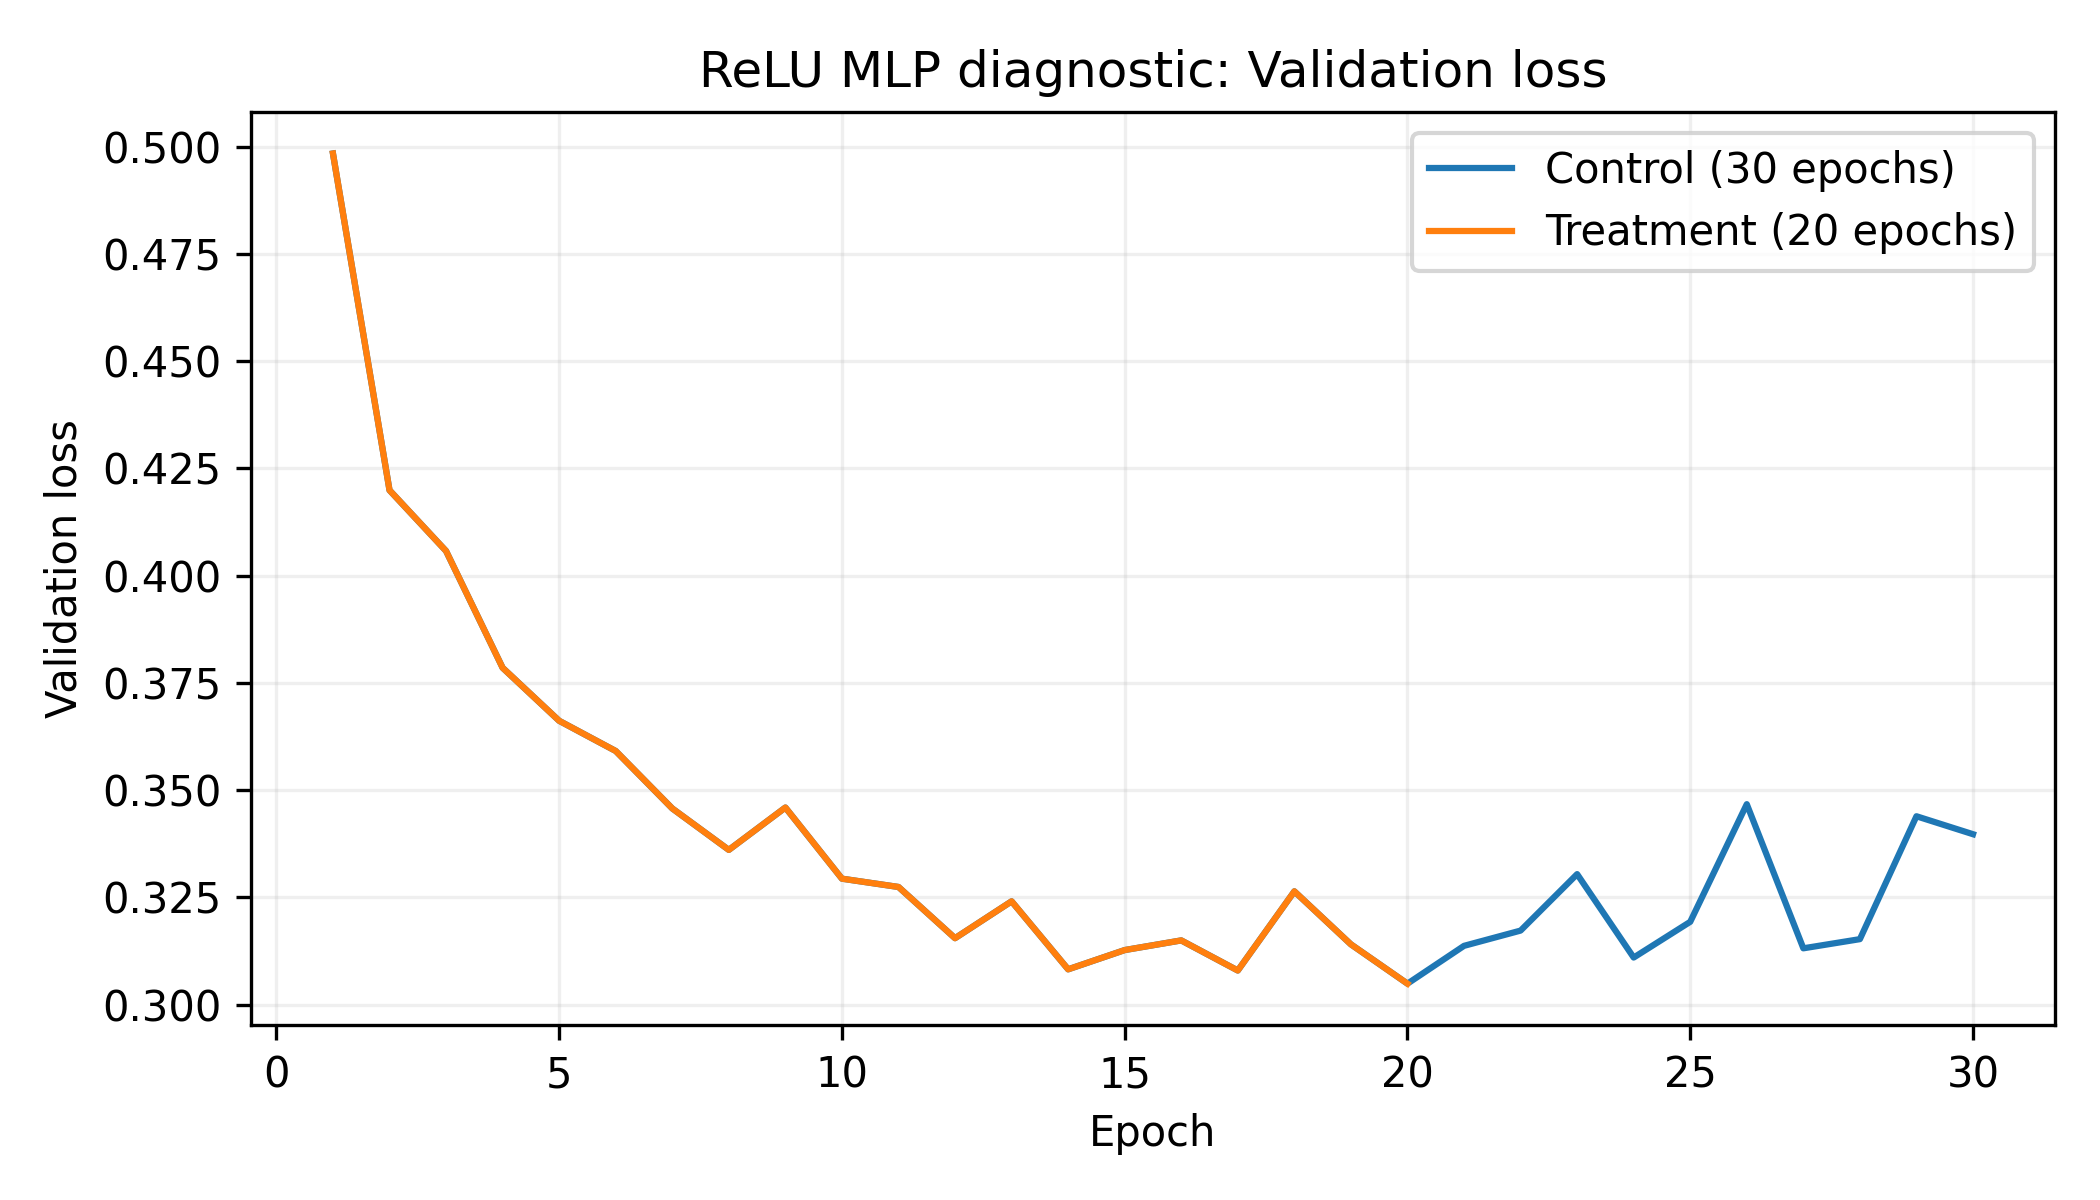
\includegraphics[width=0.93\textwidth]{images/exp1/diagnostic_val_loss.png}
\caption{ReLU MLP 训练诊断：控制组与 20 轮处理组的验证损失}
\label{fig:diagnosticloss}
\end{figure}

\begin{figure}[H]
\centering
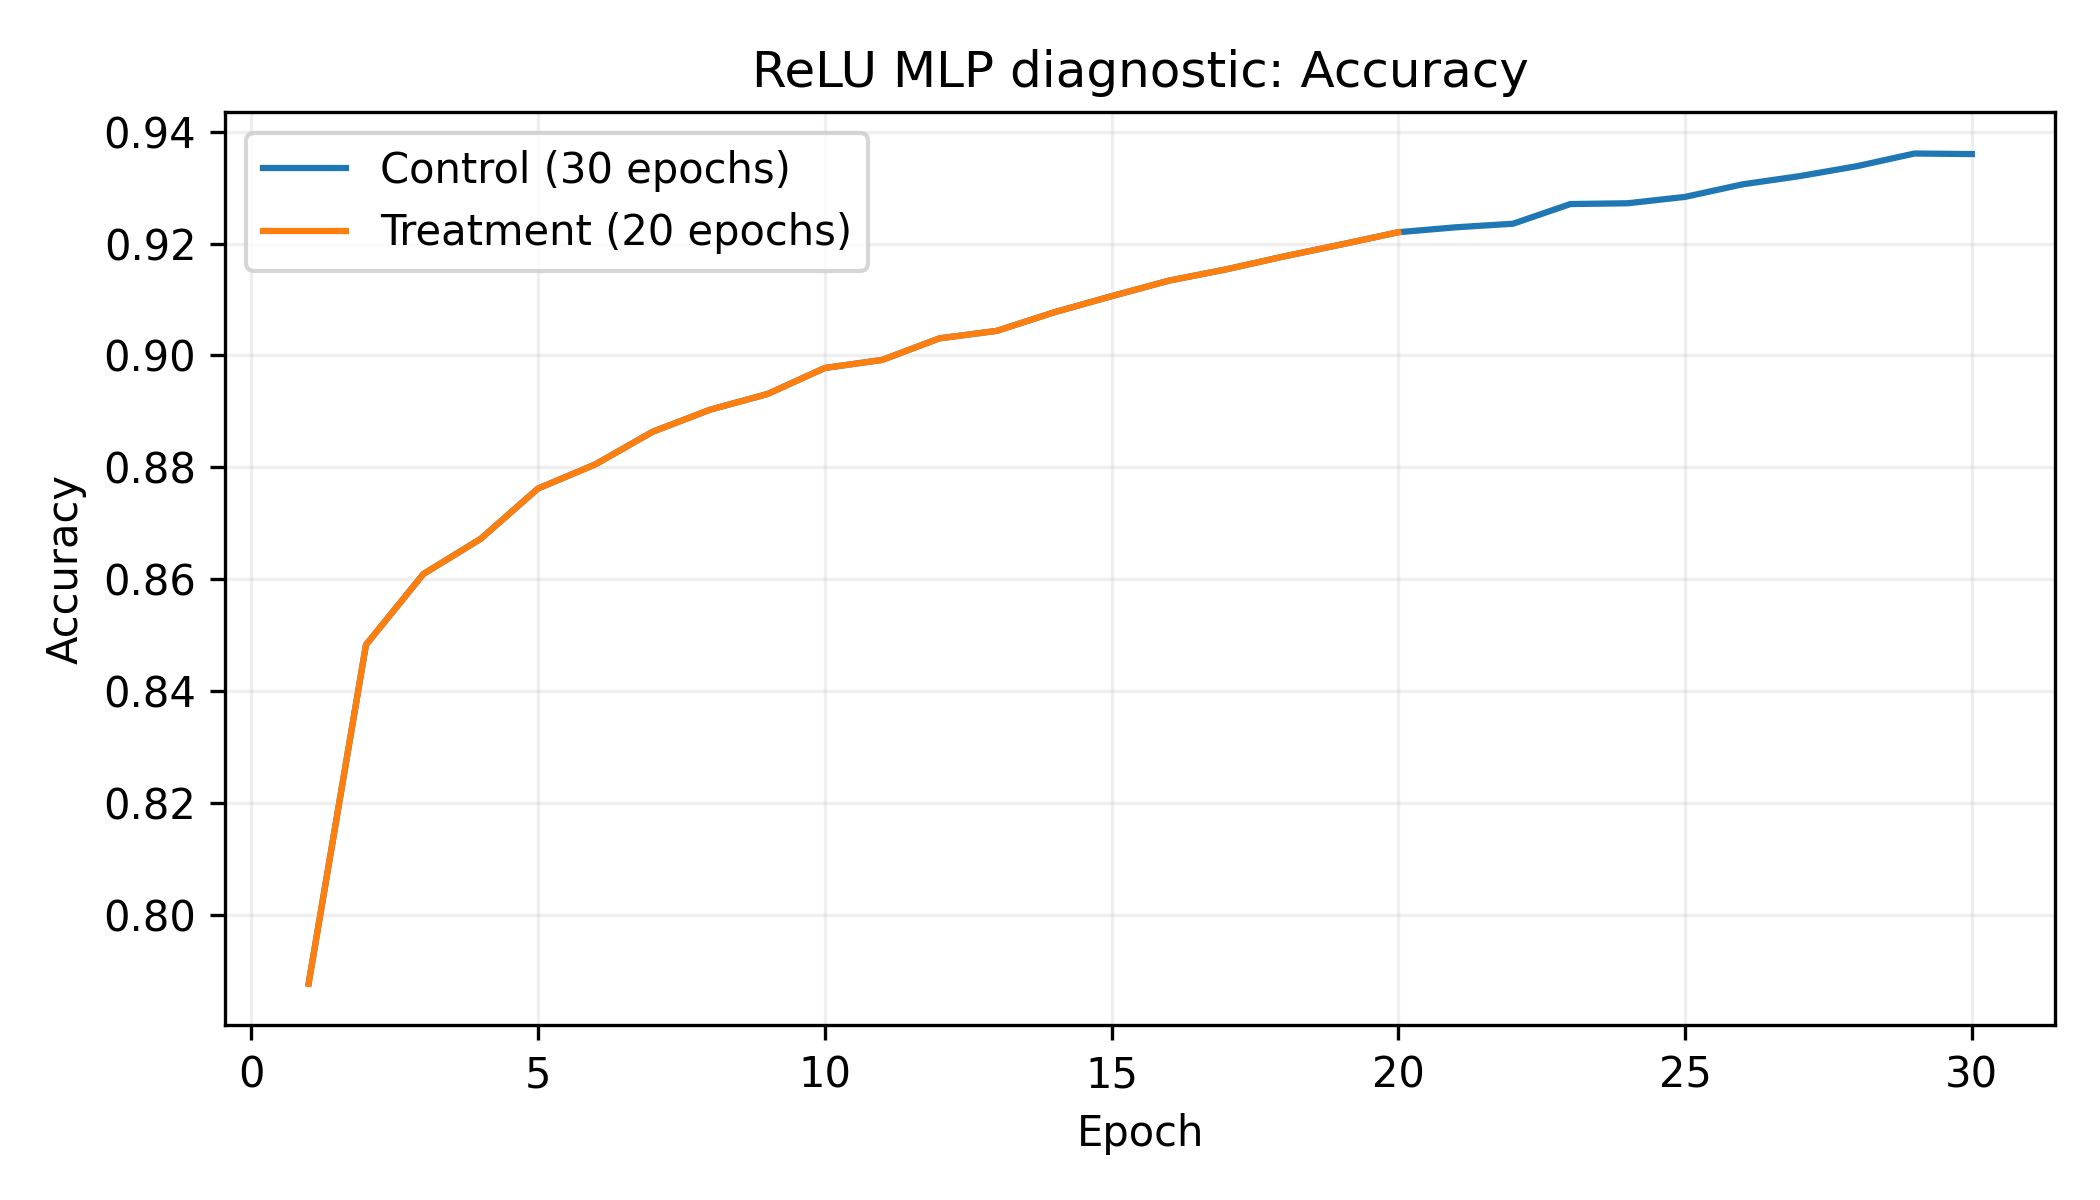
\includegraphics[width=0.93\textwidth]{images/exp1/diagnostic_accuracy.png}
\caption{ReLU MLP 训练诊断：控制组与 20 轮处理组的训练准确率（至第 20 轮重合）}
\label{fig:diagnosticacc}
\end{figure}

\section{总结与个人体会}

本实验完成了固定数据划分、线性 Softmax 基线、NumPy 手动反向传播及中心差分梯度检查，并在统一训练预算下比较了三种模型。梯度检查误差远低于阈值，为 NumPy 前向和反向实现提供了数值证据。三模型结果表明，仅增加一个无激活线性层没有带来性能提升，而 ReLU MLP 在相同数据和优化预算下获得更高的验证准确率、测试准确率和 Macro-F1。线性模型的逐类结果进一步显示，Shirt、Pullover 和 Coat 等类别较易互相混淆，符合展平线性分类器表达能力有限的特点。

训练诊断遵循了“观察问题、提出原因、只改变一个因素、用验证集作判断”的流程。缩短训练轮数获得了相近的验证表现，但收益有限；该结果提醒我应把训练集指标、验证集指标和最终测试指标分开解释，也应避免把单种子上的微小差异夸大为确定结论。

\addcontentsline{toc}{section}{参考文献}
\begin{thebibliography}{9}
  \bibitem{fashionmnist} Han Xiao, Kashif Rasul, and Roland Vollgraf. \emph{Fashion-MNIST: A Novel Image Dataset for Benchmarking Machine Learning Algorithms}. arXiv:1708.07747, 2017.
  \bibitem{project} 实验代码与复现说明：项目根目录的 \texttt{../src/}、\texttt{../numpy\_bp/}、\texttt{../scripts/}、\texttt{../configs/} 和 \texttt{../README.md}；服务器配置与逐次训练日志、汇总结果保存在本报告项目的 \texttt{work/server\_artifacts/results/} 中。
\end{thebibliography}

\end{document}
